\documentclass[output=paper]{langscibook}
\author{Stephen F. Cutler\affiliation{Cardiff University}\orcid{}}
\title[Paths to formulaicity: How do L2 speakers internalise formulaic material?]{Paths to formulaicity: How do L2 speakers internalise new formulaic material?}
\abstract{How are new formulaic expressions acquired and stored by L2 learners? Defining formulaicity with respect to the individual speaker’s storage and processing of a given expression as a single holistic unit \citep{MylesCordier2017,Wray2002}, two potential routes are explored: the ``fusion'' over time of individual words and ``holistic acquisition'', where an expression is internalised as a single unit from the start. Two studies exploring the route to acquisition are reported. L2 speakers are presented with novel target expressions to memorise, and their ease of recall, accuracy and fluency over time is monitored. These delivery features are used in combination to indicate particular stages of acquisition that may be associated with each route. Study 1 contrasts analytical and holistic methods for introducing the targets. Study 2 explores methods for determining the holisticity and processing automaticity of the target expressions in the learners’ output. Drawing on the results of these, a model for the acquisition and storage of formulaic expressions based on the ``superlemma'' model of \citet{SprengerEtAl2006} is presented and discussed in relation to fusion and holistic acquisition.}
\IfFileExists{../localcommands.tex}{
  \addbibresource{localbibliography.bib}
  % add all extra packages you need to load to this file

\usepackage{tabularx,multicol}
\usepackage{url}
\urlstyle{same}

\usepackage{listings}
\lstset{basicstyle=\ttfamily,tabsize=2,breaklines=true}

\usepackage{langsci-optional}
\usepackage{langsci-lgr}
\usepackage{langsci-gb4e}

\usepackage{todonotes}
\usepackage{siunitx}
\sisetup{group-digits=false}

\usepackage{langsci-lgr}

\usepackage[linguistics]{forest}
\usepackage{subcaption}
\usepackage{pgfplots, pgfplotstable}
\usepgfplotslibrary{colorbrewer}

  \newcommand*{\orcid}{}

\makeatletter
\let\thetitle\@title
\let\theauthor\@author
\makeatother

\newcommand{\togglepaper}[1][0]{
%   \bibliography{../localbibliography}
  \papernote{\scriptsize\normalfont
    \theauthor.
    \titleTemp.
    To appear in:
    Aleksandar Trklja \& Łukasz Grabowski.
    Formulaic language: Theories and methods.
    Berlin: Language Science Press. [preliminary page numbering]
  }
  \pagenumbering{roman}
  \setcounter{chapter}{#1}
  \addtocounter{chapter}{-1}
}

\newcommand{\researchquestion}[2]{\begin{itemize}\item[\bfseries #1]\bfseries #2\end{itemize}}


\DeclareNewSectionCommand
  [
    counterwithin = chapter,
    afterskip = 2.3ex plus .2ex,
    beforeskip = -3.5ex plus -1ex minus -.2ex,
    indent = 0pt,
    font = \usekomafont{section},
    level = 1,
    tocindent = 1.5em,
    toclevel = 1,
    tocnumwidth = 2.3em,
    tocstyle = section,
    style = section
  ]
  {appendixsection}

\DeclareNewSectionCommand
  [
    counterwithin = appendixsection,
    beforeskip=-10pt,
    afterskip=1sp,
    indent = 0pt,
    font = \usekomafont{subsection},
    level = 2,
    tocindent = 3.8em,
    toclevel = 2,
    tocnumwidth = 3.2em,
    tocstyle = section,
    style = section
  ]
  {appendixsubsection}
  
\renewcommand*\theappendixsection{\Alph{appendixsection}}
\renewcommand*{\appendixsectionformat}{\appendixname~\theappendixsection\autodot\enskip}
\renewcommand*{\appendixsectionmarkformat}{\appendixname~\theappendixsection\autodot\enskip}


\newcommand{\glossF}{\textsc{f}}
\newcommand{\glossM}{\textsc{m}}
\newcommand{\glossV}{\textsc{v}}
\newcommand{\glossN}{\textsc{n}}
\newcommand{\INSTR}{\INS}
\newcommand{\PRON}{\textsc{pron}}
\newcommand{\PREP}{\textsc{prep}}
\newcommand{\NOUN}{\textsc{noun}}
\newcommand{\PAST}{\textsc{past}}
\newcommand{\ADESS}{\textsc{adess}}
% \newcommand{\ADJ}{\textsc{adj}}
\newcommand{\CONJ}{\textsc{conj}}
\newcommand{\ESSIVE}{\textsc{essive}}
\newcommand{\GERUND}{\textsc{gerund}}
\newcommand{\NEUT}{\textsc{neut}}
% \newcommand{\NOM}{\textsc{nom}}
\newcommand{\NOUNPROPER}{\textsc{nounproper}}
\newcommand{\PART}{\textsc{part}}
\newcommand{\PRES}{\textsc{pres}}
\newcommand{\glossINF}{\textsc{inf}}
% \newcommand{\PL}{\textsc{pl}}
% \newcommand{\POSS}{\textsc{poss}}
\newcommand{\POSTP}{\textsc{postp}}
\newcommand{\PRT}{\textsc{prt}}
\newcommand{\MOD}{\textsc{mod}}
\newcommand{\NN}{\textsc{nn}}
% \newcommand{\PTCP}{\textsc{ptcp}}


\newcommand{\ESS}{\textsc{ess}}
\newcommand{\NUM}{\textsc{num}}

\newcommand{\glottocodes}[1]{}


 
  %% hyphenation points for line breaks
%% Normally, automatic hyphenation in LaTeX is very good
%% If a word is mis-hyphenated, add it to this file
%%
%% add information to TeX file before \begin{document} with:
%% %% hyphenation points for line breaks
%% Normally, automatic hyphenation in LaTeX is very good
%% If a word is mis-hyphenated, add it to this file
%%
%% add information to TeX file before \begin{document} with:
%% %% hyphenation points for line breaks
%% Normally, automatic hyphenation in LaTeX is very good
%% If a word is mis-hyphenated, add it to this file
%%
%% add information to TeX file before \begin{document} with:
%% \include{localhyphenation}
\hyphenation{
affri-ca-te
affri-ca-tes
analy-sis
}

\hyphenation{
affri-ca-te
affri-ca-tes
analy-sis
}

\hyphenation{
affri-ca-te
affri-ca-tes
analy-sis
}
 
  \togglepaper[1]%%chapternumber
}{}

\begin{document}
\maketitle 

\section{Introduction} 
\subsection{Background}

Formulaic expressions are widely used by native speakers and have been shown to bring benefits in terms of fluency and speed of processing (\citealt{Siyanova-ChanturiaSidtis2019}; \citealt{TowellEtAl1996}; \citealt{Wray2002}). The holistic nature of such expressions is thought to contribute to efficiencies in processing that enable the fluent, connected multi-clause discourse of native speakers (\citealt{PawleySyder1983}; \citealt{TremblayBaayen2010}). However, a variety of research suggests that, despite these and other benefits, L2 speakers of English do not use formulaic sequences to anything like the extent of native speakers (\citealt{Granger2019}; \citealt{Meunier2012}; \citealt{PaquotGranger2012}). Reasons given include a lack of sufficient exposure and a failure to notice that expressions may have a holistic nature. Other explanations \citep{Wray2019} are related to the different ways that native and L2 speakers may approach language learning. For example, \citet{DabrowskaLieven2005} have shown that children learn many multiword sequences as single units in their L1 and \citet{Wray2002} suggests that native speaker continue to acquire formulaic expressions as whole expressions, only later breaking them down for analysis if the need arises. On the other hand, \citet{WrayPerkins2000} have suggested that there may be a tendency for adult L2 learners to explicitly analyse any new expression in terms of its component parts. 

The extent to which L2 learners use such an approach and the effect this has on the way that formulaic expressions are internalised has not been widely researched. There are some studies (e.g. Myles, Hooper and Mitchell, 1998) which have shown that L2 learners in a classroom situation do learn and use some formulaic expressions as whole units without initially attending to their component parts. However, \citet{SchmittCarter2004} suggest that formulaic expressions are not always learnt in an all-or-nothing way. For example, studies in which L2 learners have specifically memorised sequences as whole units (\citealt{BoersLindstromberg2012}; \citealt{WrayFitzpatrick2008}) have shown that on-line reconstruction of the learned expression frequently takes place during recall and production, at least during some stages of the acquisition process. Research by \citet{Bardovi-Harlig2019} in the field of second language pragmatics proposes an acquisition process for L2 learners whereby conventional expressions go through stages of becoming more targetlike in terms of form and appropriacy to context. 

These findings suggest that the way that speakers internalise new sequences can vary. In particular, two broad routes may be hypothesised: ``holistic acquisition'', whereby a common sequence appears to be learnt and processed as a single holistic unit immediately, and ``fusion'' whereby an often used expression, initially constructed, becomes formulaic by regular usage to join the components into a single whole and fine-tune usage in terms of accuracy or appropriacy. 

This chapter explores these different possible processes for internalising the sequences through two exploratory studies in which L2 speakers memorise target multi-word sequences. The first empirical study compares two different methods of learning and measures the effect these have on how expressions become formulaic for a speaker over time. The second study further explores how formulaicity may be identified in the context of an explicit model of internal representation for formulaic expressions. Findings from these studies are brought together in a discussion of possible models of acquisition. 

\subsection{Internal formulaic expressions}\label{sec:cutler:1.2}

Many different terms and definitions have been used for formulaic language reflecting the different requirements of different schools of enquiry. An important distinction highlighted by \citet{Wray2008} is between externally-defined sequences that are considered to be formulaic ``in the language'' (such as idioms and high frequency multiword units) and those which may be ``psycholinguistic'' units in the lexicon of the individual speaker. Some researchers (\citealt{Dahlmann2009}; \citealt{Erman2007}) have shown that these are not necessarily the same, particularly for L2 speakers. For example, an L2 speaker may know of a particular idiom (which is formulaic in the language) but not be able to use it smoothly. At the same time, a specific non-idiomatic expression (such as \textit{I’m an actuary in the finance department}) may become psycholinguistically formulaic for that speaker (because it is relevant and often-repeated) while not being considered generally formulaic. \citet{TabossiEtAl2009} suggest formulaicity of an expression for an individual speaker depends on the degree of familiarity or experience with the sequence and the way it has been learned.

Formulaicity in this sense therefore relates primarily to the way a particular expression has been internalised by the individual. A useful definition for this internal formulaicity is given by \citet{MylesCordier2017}. They define an internally formulaic expression (which they term a ``processing unit'') as: 

\begin{quote}
a multiword semantic/functional unit that presents a processing advantage for a given speaker, either because it is stored whole in their lexicon or because it is highly automatised.
\end{quote}

This definition highlights the processing advantage of a formulaic expression (compared to a sequence constructed on-line) and defines the source of this to be either holistic storage in the lexicon or automaticity. The concept of holistic storage, while potentially useful as a way of representing the unitary nature of formulaic expressions, has been challenged on empirical grounds \citep{Siyanova-Chanturia2015}.  A key challenge is the finding from a variety of studies that when formulaic expressions are processed, their component words and structures are also accessed. This has been shown for idioms \citep{SprengerEtAl2006} and frequent multiword expressions \citep{ArnonPriva2014}. For example, \citet{SprengerEtAl2006} ran a series of priming experiments that analysed response times for producing idioms. These showed that idiomatic (non-compositional) sequences (e.g. \textit{hit the road}) both primed and were primed by constituent words in the sequence (e.g. \textit{road}) and that the literal word meaning of the component word becomes active during idiom production. In order to accommodate this, they propose a model where the formulaic expression is represented by a ``superlemma'' which “is a representation of the syntactical properties of the idiom that is connected to its building blocks, the simple lemmas” (p.~176) by associative links in memory. In this way, the selection and processing of an idiom is similar to the processing of a single word in terms of lexical competition and co-activation. At the same time, it retains the idea that formulaic expressions have a syntactic structure related to the individual constituents at the lexico-syntactic level. This model therefore provides a good starting point for exploring the acquisition of internal formulaic expressions and is described in more detail in \sectref{sec:cutler:3.2}.

\subsection{Exploring acquisition through targeted memorization}\label{sec:cutler:1.3}

A useful way to investigate the acquisition of internal formulaic expressions by L2 speakers is through the targeted memorisation of novel expressions. Variations on such an approach have been used by \citet{Wray2004} and \citet{FitzpatrickWray2006} although not with a specific focus on internal formulaicity. In order to extend the targeted memorisation approach to investigate different paths to formulaicity, it is necessary to establish a way of identifying formulaicity in spoken output. Although it is not possible to observe cognitive attributes such as holistic storage or automatization directly, a common approach for identifying formulaicity has been to use sequence fluency. For example, in studies by \citet{Erman2007} and \citet{Dahlmann2009}, the absence of disfluency markers (such as pauses, hesitation, and repetition) was used as a criterion for formulaicity. More recently, \citet{MylesCordier2017} have developed a set of criteria for the internal formulaicity of a sequence whereby fluency (indicating phonological coherence) along with evidence of its unitary nature (such as grammatical irregularity or semantic opacity) are the two necessary conditions. A sufficient criterion for satisfying the second condition is that the learner has experienced the sequence as a unitary form with a given meaning. Therefore, in the specific case of targeted memorisation, the approach of \citet{MylesCordier2017} effectively equates internal formulaicity with consistent fluency of delivery of the sequence at the time of testing.

The memorisation study by \citet{FitzpatrickWray2006} highlighted considerable individual differences between participants in how they approached the process of memorising target sequences. Choosing how to control the input method is therefore an important consideration, since it is likely to have a significant effect on the learning outcome. For example, the principle of transfer appropriate processing \citep{RoedigerEtAl2002} proposes that any processing strategy is linked to a particular outcome. \citet{Craik2002} states that encoding and retrieval are integrated in such a way that the initial processes determine the qualitative nature of the trait encoded. \citet{Barcroft2002, Barcroft2006}, exploring processing specificity, has shown that semantic, formal and mapping components are three separate and dissociable processes, and focusing on any one may take resources from the others. In general, elaborative approaches (strategies that facilitate an increased evaluation of an item with respect to particular features such as its meaning or structure) have been shown to increase learning with respect to that feature. For the intentional learning of formulaic expressions, different forms of semantic or formal elaboration have been suggested. These include: drawing attention to L1 congruence (\citealt{ConklinCarrol2019}), analysing component words and structure through matching or cloze style activities \citep{BoersEtAl2014}; linking metaphorical meanings of non-compositional idioms \citep{BoersEtAl2007}; and utilizing imageability \citep{SteinelEtAl2007}. These may lead to learning benefits in terms of long-term recall and accuracy, but their effect on fluency is not clear.

Insofar as internal formulaicity is defined in terms of holisticity and identified by delivery features such fluency, approaches to memorisation that are geared towards this outcome may be more effective in promoting ``holistic acquisition''. A key means of achieving fluency in a targeted sequence has been shown to be oral repetition. For example, \citet{Nelson1977} demonstrated that repetition “at the phonemic depth of processing” facilitates memory for cued and un-cued recall and for recognition. \citet{YoshimuraMacWhinney2007} showed that oral production fluency increases with the number of repetitions. The way in which the repetition is conducted is also important. Research into the effective learning processes of Chinese students (\citealt{AuEntwhistle1999}) suggests that rote memorisation is more effective if it is accompanied by a link with meaning. A study by \citet{Ding2007} reported that a learning task involving the memorisation of a film script by copying a DVD was effective because the learners were being fully attentive to an imitation process. \citet{NoiceNoice2006} researched how actors are able to learn their lines. They showed that, for the non-actors participating in their study, the strategy of ``actively experiencing'' the line as it was being spoken was more effective for accurate, fluent recall and reproduction than other memorising strategies. These kinds of repetition strategy may therefore be appropriate for achieving accurate acquisition of the complete phonological form while at the same time providing a strong automatic link to overall meaning and context. 

\section{Study 1: Comparing paths to formulaicity}
\subsection{Overview} 

The first study explores possible routes towards internal formulaicity by having L2 speakers memorise new target sequences via two different approaches. The first, Dynamic Repetition (DR), focuses on accurate and fluent reproduction of the sequences, while the second, semantic-formal elaboration (SFE), is a more elaborative approach focusing on meaning and form. The effect of these initial processing strategies on formulaicity is assessed over time in terms of the fluency and accuracy with which the expressions are recalled. 

Following the approach of Myles and Cordier (2017) as outlined in \sectref{sec:cutler:1.3}, internal formulaicity is indicated by the fluent delivery of the target sequence on recall. On this basis, it was hypothesised that the DR approach to learning was more likely to induce  ``holistic acquisition'' (as indicated by a target becoming internally formulaic immediately after initial learning).

After the initial learning phase, accuracy and fluency of recall were also tested after one and three weeks using a controlled series of recall tasks. As well as a means for checking internal formulaicity over time, these were designed to provide additional practice of the targets in a consistent way, allowing for the possibility of acquisition by ``fusion'' (as indicated by a target becoming formulaic at a later stage). 

\subsection{Method}
\subsubsection{Participants}

Ten Japanese speakers of English (JSE) at an intermediate/advanced level of English were recruited. There were nine females and one male, with ages from 28 to 45 and recent TOEIC scores \citep{ETS2019} ranging from 760 to 940. All were working adults chosen based on availability, level and because they were interested to take part. Full ethical procedures were followed in the collection of data and pseudonyms used when reporting on individual contributions. 

\subsubsection{Design}

The target sequences to be memorised are listed in \tabref{tab:cutler:1}. All were verb phrases of 4 or 5 words selected from the Phrases in English (PIE) on-line corpus \citep{Fletcher2011}. Each had high frequency lexical words (with no repetition of these across the sequences), was non-congruent with the L1 Japanese. The sequences were confirmed to be unknown to the participants via an on-line check which involved them completing a cloze-style test and a check of recognition. The sequences were embedded in 4 stories (each of about 150 words) and the stories were paired to form two sets (AB and CD) of 6 sequences each. Sequences were balanced across the sets for length (words and syllables). Each story was assigned a suitable picture as a visual cue.


\begin{table}
\begin{tabular}{ll}
\lsptoprule
\multicolumn{2}{c}{Set 1 (AB)}\\\midrule
A1 & turned a blind eye to\\
A2 & came to a head\\
A3 & breathed a sigh of relief\\
B1 & run the risk of\\
B2 & go a long way towards\\
B3 & like the sound of\\\midrule
\multicolumn{2}{c}{Set 2 (CD)}\\\midrule
C1 & set his sights on\\
C2 & stood the test of time\\
C3 & get the hang of\\
D1 & knew better than to\\
D2 & toyed with the idea of\\
D3 & remains to be seen\\
\lspbottomrule
\end{tabular}
\caption{List of target sequences\label{tab:cutler:1}}
\end{table}


To mitigate against the possible confounding effect of differences between participants or sequence memorability, a cross-over design was used whereby participants, sequences and order of learning were balanced across the two conditions. To facilitate this, participants were randomly assigned to one of four groups, as shown in \tabref{tab:cutler:2}.


\begin{table}
\begin{tabular}{lll} 
\lsptoprule
  & 1st & 2nd\\\midrule
P1& AB (DR) & CD (SFE)\\
P2& AB (SFE) & CD (DR)\\
P3& CD (DR) & AB (SFE)\\
P4& CD (SFE) & AB (DR)\\
\lspbottomrule
\end{tabular}
\caption{Ordering of sequences and conditions by participant group\label{tab:cutler:2}}
\end{table}

\subsubsection{Procedure}

Each participant listened to a story (A or C) without any script, but while looking at the picture (to provide a cue for later). The three sequences in that story were introduced for learning either using DR or SFE (described below). The process was repeated for the second story (B or D), using the same method. The six sequences were then tested for recall (see \sectref{sec:cutler:2.2.4}). Next the procedure was repeated for the other two stories, with the sequences learned using the other method. The time given for memorisation of targets was the same for both conditions (18 minutes for 6 sequences). After all sets had been learnt and assessed, the participants listened to each story once more. Following a 10-minute break, there was a further assessment to establish performance at the end of the learning session (W0). After one week and three weeks, participants were given further assessments (W1 and W3 respectively).

The input sessions varied according to the condition as follows.

\subsubsubsection{DR input} 

DR input approach focusses on consistent repetition of the expression with an emphasis on accurate imitation of prosody, intonation and rhythm, and ``active experiencing'' of the sequences. The basic meaning of the expressions is provided by the story and the translations but is not further elaborated on. For each sequence, participants listened to the full sentence containing it and read a translation to check meaning. They then did a series of repetitions of the sequence following the exact intonation and rhythm of the model provided. (Where necessary this was slowed down to ensure accuracy). They interspersed this with repeating the whole sentence and also practised responding quickly to the Japanese translation of the sequence (as a cue card). Participants were encouraged to mimic the exact prosody and intonation of the delivery whenever they repeated each expression and “to imagine they were performing in a radio play”. All engaged willingly with the process and appeared to enjoy doing it.

\subsubsubsection{Semantic/formal elaboration (SFE) input} 

SFE consisted of a generative exercise followed by some form-meaning tasks relating to the components, structure and meaning of the sequence. After listening to the story, participants were given a gap fill exercise based on the story script to try to generate the sequences. After finishing, they corrected this using the answer script and repeated each sequence out loud. They then did exercises looking at the structure of each sequence (count the verbs and nouns) and compared the sequence with its Japanese translation by rating their ``closeness'' (in terms of words used). They were also asked to consider what might help them remember each sequence (e.g. particular words or images) and wrote example sentences for each which were then corrected if necessary by the researcher.

\subsubsection{Assessments and measures}\label{sec:cutler:2.2.4}

The same set of assessment tasks was applied at all stages:

\begin{description}
\item[Context recall:] Given the picture and title, the participant retells the story trying to use the target expressions. 
\item[Cued recall:] Cue cards (featuring the L1 translation of each sequence) are presented in random order and the participant recalls the appropriate sequence out loud. If they cannot do so, the researcher says the first word as a further cue. 
\item[Written recall:] Participant writes down the expressions given the L1 translation
\item[Read out loud:] Each target is presented on a computer screen in random order and the participant repeats it.
\end{description}

The assessments were recorded, transcribed and analysed to calculate a variety of measures for each participant-sequence. For reasons of space, the current report focuses only on the context and cued recall tasks and on the following measures:

\begin{description}
\item [Recall:] The sequence was deemed to have been recalled if over 70\% of the words matched the target on either of the recall attempts (context or cued). 
\item [Accuracy:] The sequence was considered ``fully accurate'' if it exactly matched the target on either of the recall attempts. 
\item [Fluency:] For each recall attempt, any pause ($>0.2\text{s}$), reformulation, filler or hesitation was marked as a dysfluency. The sequence was considered ``consistently fluent'' if it was delivered with no dysfluencies and with consistent form across the recall attempts. 
\end{description}

The context and cued recall tests provide two different opportunities for the participants to recall and speak the expressions. The measures here are based on the combined responses to both tasks.

\subsection{Results and key points}
\subsubsection{Summary of results}


Overall, the ten participants, each learning six sequences via DR and six via SFE provided 120 participant-sequence combinations (60 for each condition). The numbers of sequences that are recalled (R-\#), fully accurate (A-\#) and consistently fluent (F-\#) by condition and assessment phase across the two conditions at each of the assessments are given in \tabref{tab:cutler:3}.  The table also gives the cross-participant mean proportion of recalled sequences that were consistently fluent (Mean-F)

\begin{table}
\begin{tabular}{llrrrc}
\lsptoprule
Phase & Cond & \multicolumn{1}{c}{R-\#} & \multicolumn{1}{c}{A-\#} & \multicolumn{1}{c}{F-\#} & Mean-F\\\midrule
W0  & {DR}  & {47/60 (78\%)} & {39/60 (65\%)} & {19/47 (40\%)} & {0.458 (sd=0.244)}\\
    & {SFE}  & {52/60 (87\%)} & {39/60 (65\%)} & {11/52 (21\%)} & {0.215 (sd=0.152)}\\
W1  & {DR}  & {39/60 (65\%)} & {33 (55\%)} & {15/39 (38\%)} & {0.398 (sd=0.314)}\\
    & {SFE}  & {37/60 (62\%)} & {23/60 (38\%)} & { 7/37 (19\%)} & {0.167 (sd=0.236)}\\
W3  & {DR} & {49/60 (82\%)} & {40/60 (67\%)} & {21/49 (42\%)} & {0.448 (sd=0.233)}\\
    & {SFE}  & {50/60 (83\%)} & {39/60 (65\%)} & {12/50 (24\%)} & {0.258 (sd=0.262)}\\
\lspbottomrule
\end{tabular}
\caption{Recall, accuracy and fluency by condition and assessment phase\label{tab:cutler:3}}
\end{table}


The initial effect of the two input methods can be seen in the results immediately after learning (W0). These show that recall is slightly better for sequences learnt via SFE, while accuracy is similar across the two condition. For fluency, the proportion of recalled sequences that are consistently fluent (F-\#) is higher in the DR condition (40\%) than in SFE (21\%). This difference is also evident in the Mean-F scores.  A Wilcoxon signed-rank test indicated that the proportion of fluent sequences for the DF condition at W0 was significantly higher than for the SFE condition ($Z=-2.801, p=0.00256$).

For the subsequent assessments, the general pattern of results for recall, accuracy and fluency is for a dip from W0 to W1 followed by a return to earlier levels at W3. This can be seen graphically in \figref{fig:cutler:1}.


\begin{figure}
\begin{tikzpicture}
\begin{axis}[
      name = first,
      width = .33\textwidth,
      title = {Recalled (R-\#)},
      symbolic x coords = {W0,W1,W3},
      xtick=data,
      ymin = 0,
      ymax = 100,
      cycle list/Set1-3,
    ]
    \addplot+ [mark=square*] coordinates {
        (W0, 78)
        (W1, 65)
        (W3, 82)
    };
    \addplot+ [mark=*] coordinates {
        (W0, 87)
        (W1, 62)
        (W3, 83)
    };
\end{axis}%
\begin{axis}[
      name = second,
      at = (first.right of east), 
      xshift = 1cm,
      anchor=west,
      width = .33\textwidth,
      title = {Accurate (A-\#)},
      symbolic x coords = {W0,W1,W3},
      xtick=data,
      ymin = 0,
      ymax = 100,
      cycle list/Set1-5,
    ]
    \addplot+ [mark=square*] coordinates {
        (W0, 65)
        (W1, 55)
        (W3, 67)
    };
    \addplot+ [mark=*] coordinates {
        (W0, 65)
        (W1, 38)
        (W3, 65)
    };
\end{axis}%
\begin{axis}[
      at = (second.right of east),
      xshift = 1cm, 
      anchor= west,
      width = .33\textwidth,
      title = {Fluent (F-\#)},
      symbolic x coords = {W0,W1,W3},
      xtick=data,
      ymin = 0,
      ymax = 100,
      cycle list/Set1-5,
      legend pos = outer north east
    ]
    \addplot+ [mark=square*] coordinates {
        (W0, 40)
        (W1, 38)
        (W3, 42)
    };
    \addlegendentry{DR}
    \addplot+ [mark=*] coordinates {
        (W0, 21)
        (W1, 19)
        (W3, 24)
    };
    \addlegendentry{SFE}
\end{axis}
\end{tikzpicture}
\caption{Proportions of recalled, fully accurate and consistently fluent sequences by condition and assessment phase\label{fig:cutler:1}}
\end{figure}


\subsubsection{Evidence of holistic acquisition and fusion}
Following the approach of \citet{MylesCordier2017}, fluent, consistent delivery of a sequence is considered a potential indicator of its internal formulaicity for that speaker. F-\# therefore provides a count of such sequences. At W0, immediately after learning, the proportion of fluent targets was significantly higher for sequences learnt via DR than for those learnt by SFE, suggesting that the DR input did support holistic acquisition and may result in more expressions becoming formulaic for the speaker straight away. At the same time, this method did not appear to have a detrimental effect on recall or accuracy of the learnt expressions. However, while around 80\% of the sequences were recalled at W0, even in the DR condition only about 40\% of these were fully fluent. This may indicate limits on the numbers of sequences that can be memorised holistically in the given time period.

The results for the subsequent assessments suggest that similarities and differences between the conditions tended to remain over the three weeks. In particular, the proportion of fluent sequences for DR was still greater than that of SFE at W3. Although the overall numbers are small, the trend seems to suggest that the beneficial effects of DR are maintained over the longer term. On the other hand, the fact that the actual number of fully fluent sequences did not change much between W0 and W3, suggests that few additional sequences became formulaic for the speakers over the three weeks. For most targets, a reconstructive approach continued to be applied during recall. A typical pair of responses is given in \REF{ex:cutler:1}, where there is increased fluency and accuracy at W3, but without yet being sufficient for the target to be considered internally formulaic for the speaker.


\ea Context recall responses by Kentaro for \textit{breathed a sigh of relief} (``/'' indicates points of dysfluency).\label{ex:cutler:1}\smallskip\\
\begin{tabularx}{\linewidth}{@{}lQ@{}}
W0 & he breathe on\slash breathe a\slash this one he breathe something\slash breathe\slash sigh\slash of relief\slash that …\\
W3 & he breathed\slash a\slash bre- breathed a sigh of relief\slash because …\\
\end{tabularx}
\z


It may be that the earlier assessment tasks at W0 and W1 (the only way the speakers had to ``practice'' the expressions) were not sufficient to move more sequences into formulaicity at W3, but further practice could do so. 

\subsubsection{Overall recall performance over time}\label{sec:cutler:2.3.3}
The overall pattern of performance in recall and accuracy of the target sequences was for a reduction in week 1 followed by an improvement in week 3. Since all participants confirmed that (as instructed) they had not reviewed the targets between tests, the overall reduction in performance at W1 is a not unexpected decay. However, the increased recall accuracy and fluency at W3 is more surprising. Since the only additional learning or review of the sequences following the initial input session was the W1 assessment check, the week 3 results suggest that this influenced the long-term learning. This interpretation supports work on spaced retrieval \citep{KornellEtAl2015} which suggests that recall of learnt items (e.g. words learnt via flash cards) is enhanced by each attempt to retrieve them, and this effect occurs whether or not that attempt is successful, provided the correct answer is subsequently given. Although their work was not specifically on the learning of sequences, the retrieval conditions in the assessments used here were comparable. So, the repeated assessments may have supported the enhanced performance at week 3 as this was the fourth time the sequences were retrieved. Further, since the two retrieval attempts preceding W3 (W0 and W1) were spaced by a week while those preceding W1 were only spaced by 20--30 minutes in the initial session, the results may support research (\citealt{KornellVaughn2016}) that claims increasing retrieval spacing has a beneficial effect on learning. 

\section{Study 2: Exploring fluency and holistic automaticity}
\subsection{Introduction}

While using fluency as an indicator of formulaicity follows a precedent set by previous research, it may be argued that fluency alone does not always imply holistic storage or automatic processing of the sequence (the defining features of internal formulaicity in the definition of \citealt{MylesCordier2017}). For example, \citet{Segalowitz2010} argues that automaticity is more than a simple speeding up of cognitive processes; it involves a qualitative change in the way a process is organised or structured. Establishing a form of internal holisticity may represent such a qualitative difference for formulaic sequences when compared with simply constructing the sequence more and more fluently through repetition. Segalowitz describes a type of automaticity linked with qualitative restructuring, terming it ``ballistic automaticity'', based on the idea of automatic processing being unstoppable or involuntary. 

Study 2 explores the idea that fluency may be a staging post towards formulaicity rather than necessarily the destination. Drawing together the ballistic automaticity described by \citet{Segalowitz2010} and the representation of internal holisticity given by the model of \citet{SprengerEtAl2006}, a psycholinguistic test for \textit{holistic automaticity} was used to determine the formulaicity of target sequences more explicitly. This was then applied to new data from the same group of 10 Japanese speakers of English who took part in Study 1. The aim was to determine the extent to which target sequences that are delivered consistently and fluently can also be shown to be automatic and holistic in the mind of the speaker. It also offered the opportunity to further explore the route to formulaicity of the original sequences. 

\subsection{Holistic automaticity test}\label{sec:cutler:3.2}

In Holistic automaticity (HA), when the first word of a target sequence is activated (by hearing the word as an auditory prime), the speaker cannot help but process the whole sequence for potential speech production. In particular, subsequent words in the sequence will be activated and, given a suitable cue, preferentially selected over other candidate words in a word response test. The reasoning for this draws on the amended hybrid model of speech processing of \citet{SprengerEtAl2006} introduced in \sectref{sec:cutler:1.2}.

\begin{figure}
\caption{Adapted version of ``superlemma'' model \citep[1760]{SprengerEtAl2006}. Arrows with filled heads show meaning relationships, those with non-filled heads show associative links\slash co-activation.\label{fig:cutler:2}}
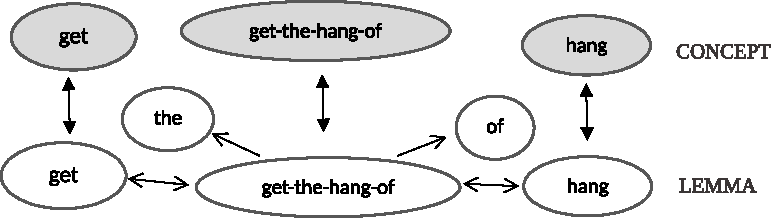
\includegraphics[width=\textwidth]{figures/cutlerFig2.pdf}
\end{figure}

\figref{fig:cutler:2} shows a simplified version of the model as applied to a target sequence from the current study. If the sequence is formulaic, the contention is that a superlemma (\textit{get-the-hang-of)} exists which is linked to both to its conceptual meaning directly and to the lemmas of its constituent words via associative link. When the identity prime (\textit{get}) is heard, the lemma for \textit{get} is activated which then activates the lemma for \textit{get-the-hang-of}. This in turn activates the other constituent word lemmas, including the lemma for \textit{hang}. When the letter cue (h\_) is then seen, it triggers a search for words beginning with h. Since \textit{hang} is already active, selection of this word is facilitated above other candidates.

\subsection{Method}
\subsubsection{Target sequences}


Along with the 12 sequences previously learnt by the participants in Study 1, six new control sequences were introduced. These were selected using the same principles as the originals and confirmed to be unknown to the participants. 

For the HA testing, the initial verb of the sequence was taken as the prime and one of the key lexical words in the remainder of the sequence was the target word. For example, for the sequence \textit{get the hang of}, \textit{get} was the prime word and \textit{hang} the target. Each sequence was to be presented twice: once with a cue letter corresponding to the target word (T-cue), once with a cue letter unconnected to the sequence (NT-cue). The list of sequences, primes and cue letters is given in \tabref{tab:cutler:Appendixtable}.

\begin{table}
\caption{List of target sequences, primes, cues and target words for the HA Test (Study 2). Note: A1--D3 are the original sequences; E1--F3 the new controls\label{tab:cutler:Appendixtable}}
\begin{tabular}{llllll}
\lsptoprule
   & Sequence & Prime & T-cue & Target & NT-cue\\\midrule
A1 & turned a blind eye to & turned & b & blind & f\\
A2 & came to a head & came & h & head & b\\
A3 & breathed a sigh of relief & breathed & r & relief & t\\
B1 & run the risk of & run & r & risk & l\\
B2 & go a long way towards & go & l & long & s\\
B3 & like the sound of & like & s & sound & t\\
C1 & set his sights on & set & s & sights & t\\
C2 & stood the test of time & stood & t & test & i\\
C3 & get the hang of & get & h & hang & r\\
D1 & knew better than to & knew & b & better & r\\
D2 & toyed with the idea of & toyed & i & idea & l\\
D3 & remains to be seen & remains & s & seen & l\\
E1 & look on the bright side & look & b & bright & f\\
E2 & rolls off the tongue & rolls & t & tongue & h\\
E3 & scared the life out of & scared & l & life & h\\
F1 & walk on thin ice & walk & i & ice & s\\
F2 & reserve the right to & reserve & r & right & i\\
F3 & lie at the heart of & lie & h & heart & f\\
\lspbottomrule
\end{tabular}
\end{table}

\subsubsection{Procedure}
\subsubsubsection{Fluency assessment}
To determine the current state of acquisition of the 12 sequences each participant undertook the same assessment (context recall and cued recall) given in Study 1. On this basis, participant-sequences were categorised into one of the following:

\begin{enumerate}
\item No recall (NoRec): The sequence was not recalled with sufficient accuracy in either task
\item Major dysfluency (D-major): Major or multiple disfluencies in either task
\item Minor dysfluency (D-minor): Only one minor disfluency in one or both tests
\item Fluent, low recall (F-low): Recalled on one test and fully fluent in that one
\item Fluent, high recall (F-high): Recalled on both tests and fully fluent and consistent in both
\end{enumerate}

This categorisation was chosen to separate out those sequences that were judged phonologically coherent for that speaker at that time (4, 5) from those that were not (1, 2, 3). In addition, it enabled exploration of the extent to which ease of recall (of the whole sequence) and the ``degree'' of fluency of a sequence may be relevant to automaticity. A minor dysfluency was defined as a single short pause (between 0.2s and 0.5s) occurring in one or both of the tests.

\subsubsubsection{Brief review of the sequences}
Following the assessment, the six control sequences were read out to the participant and then shown on a written list with a Japanese translation. The participant read each one out loud once to ensure it could be said smoothly with no pronunciation difficulties. After a short break, the participant was presented with all 18 target sequences in random order and asked to read each one out loud (to integrate the controls into the set of targets). 

\subsubsubsection{Introduction of response word controls}
To provide some degree of control over the possible responses, a set of 40 words was introduced before the test. This was considered necessary to reduce the possibility that target words are chosen simply because of exposure to the target sequences during the earlier stages of the experiment. The 40 words contained 8 different starting letters which matched the range of cue letters of the test. All 18 target words were included along with 22 high frequency dummy words of similar form, resulting in 5 words for each initial letter. 

Participant were presented with the words one-by-one on cards in random order. After repeating each one out loud, they performed a simple grouping exercise based on initial letter and repeated them again. After a break and immediately prior to the holistic test, a brief check was done in which the participants were presented with each cue letter and asked to say out loud any word they could think of. The purpose of this was to ascertain whether target words were preferentially in mind before the test. 

\subsubsubsection{HA test and analysis}
The computer-based HA test consisted of 36 items (two for each target sequence). For each item, there was a fixation point on the screen accompanied by a beep. After 2.5s an auditory prime of the cue word (the first word of a sequence) was played and a further 750ms later, the cue letter appeared. Each spoken prime lasted between 500--600ms, leaving a short gap (150--250ms) before the letter cue was shown. The 36 items were presented in pseudo-random order to ensure that: (a) the two occurrences of each sequence were well separated, (b) the same cue letter was not repeated sequentially, and (c) cue letters did not follow presentation of a prime word with the same beginning letter. This was to minimise cross-item interference. Participants were given the following instruction: 

\begin{quote}
You will hear a word. You will then see a letter. Say a word beginning with that letter as quickly as you can. NOTE: You may like to use one of the words introduced earlier but you don’t have to. The aim is to respond as quickly as possible
\end{quote}

The aim was to encourage participants to choose words from the list but without compelling them to think too consciously about it. Each test was recorded, and the participant response and response time (RT) noted for each item. To determine whether the target word had been activated and spoken quickly and in preference to other possibilities, a set of criteria was applied for each target sequence:

\begin{itemize}
\item The expected target word must be chosen in response to the T-cue.
\item The RT for this word should be faster than that for the NT-cue word for the same prime.
\item If there are other occasions when the same target word is given (i.e. as an NT-cue response to a different prime), all of these should also have slower RTs.
\end{itemize}

If all criteria were satisfied for a sequence for the participant, it was marked as a ``holistic hit''. To illustrate, \tabref{tab:cutler:5} gives a typical example of a possible set of participant responses involving the prime \textit{get} and the response \textit{hang} (for testing the sequence \textit{get-the-hang-of}). In this example, the appropriate target response is given, and its RT is faster than any other response involving the prime \textit{get} or the response \textit{hang}. So, it would be marked as a holistic hit.


\begin{table}
\begin{tabular}{lllr}
\lsptoprule
Prime  & Cue & Response & RT (s)\\\midrule
get & h\_ & hang & 1.125\\
get & b\_ & boy & 1.491\\
lie & h\_ & hang & 1.662\\
rolls & h\_ & hang & 2.010\\
\lspbottomrule
\end{tabular}
\caption{Example holistic test responses\label{tab:cutler:5}}
\end{table}

\subsection{Results}

Across the ten participants, a total of 49 of the original sequences were deemed to be formulaic (23 low recall and 26 high recall), while 56 were non-formulaic (38 with major dysfluencies, 18 with a minor dysfluency) and 15 were not recalled at all. This information was used to divide the results into categories for subsequent analysis.

In the word check test, 61\% of responses were from the list of 40 control words given at the start of the session. Of these, 34\% were target words from the original sequences and 16\% were target words from the control sequences. These figures are close to the percentages expected if the words were chosen at random (12/40=30\% and 6/40=15\%, respectively). This was the anticipated result and confirmed that the target words were not preferentially activated before the test compared to other possible choices of words.


% % % \begin{table}
% % % \begin{tabularx}{\textwidth}{XXXXXX}
% % % \lsptoprule
% % % \multicolumn{2}{c}{{\bfseries Sequence type}} & \multicolumn{2}{c}{{\bfseries N}} & \multicolumn{2}{c}{{\bfseries Holistic Hits}}\\
% % % \multicolumn{2}{c}{Control} & \multicolumn{2}{c}{60} & \multicolumn{2}{c}{9 (15\%)}\\
% % % \multicolumn{2}{c}{Not recalled} & \multicolumn{2}{c}{15} & \multicolumn{2}{c}{2 (13\%)}\\
% % % Dysfluent & Major & 38 & 56 & 8 (21\%) & 15 (26\%)\\
% % % & Minor & 18 &  & 7 (39\%) & \\
% % % Fluent & Low recall & 23 & 49 & 12 (52\%) & 31 (63\%)\\
% % % & High recall & 26 &  & 19 (73\%) & \\
% % % \lspbottomrule
% % % \end{tabularx}

\begin{table}
\begin{tabular}{lrrrrcrrc}
\lsptoprule
    & Control & NR & \multicolumn{3}{c}{Dysfluent} & \multicolumn{3}{c}{Fluent}\\\cmidrule(lr){4-6}\cmidrule(lr){7-9}
    &         &              & Major & Minor & Σ             & Low recall & High recall & Σ\\\midrule
$N$ & 60      & 15           & 38 & 18 & 56                  & 23 & 26 & 49\\ 
HH  & 9       & 2            & 8  & 7  & 15                  & 12 & 19 & 31\\
\%HH& 15      & 13           & 21 & 39 & 26                  & 52 & 73 & 63\\\lspbottomrule
\end{tabular}
\caption{Proportion of holistic hits over main categories. NR: Not recalled; HH: Holistic hits.\label{tab:cutler:6}}
\end{table}

\tabref{tab:cutler:6} gives the numbers and proportions of holistic hits across the sequence categories. As the table shows, the memorised sequences deemed formulaic by the criteria had a much higher percentage of holistic hits compared with non-formulaic learned sequences. The control sequence results are similar to those of the original sequences which were not recalled. Excluding the No Recall group, a chi-square analysis comparing counts for Control, Non-F and Formulaic groups shows that the differences are significant ($\chi^2=25.257, p<0.00001$) with Cramér's  $V=0.28$, suggesting a medium to large effect \citep{Cohen1988}.

Looking at the more detailed categories, the proportion of holistic hits rose steadily from major dysfluency to minor dysfluency to fluent. Within sequences categorised as fully fluent, it rose from low recall to high recall. The results are suggestive that the likelihood of a sequence being holistically automatic increases the more fluent it appears to be and the more easily it is recalled. \figref{fig:cutler:3} summarises the results, showing the continuous rise in holistic hits (representing holistic automaticity) through the categories (representing increasing degrees of fluency).

\begin{figure}
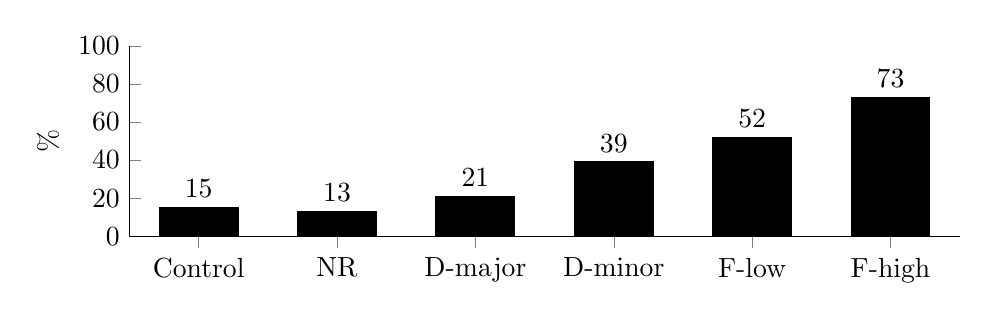
\begin{tikzpicture}
  \begin{axis}[
      ybar,
      ymin=0,
      ymax=100,
      xtick=data,
      symbolic x coords = {Control, NR, D-major, D-minor, F-low, F-high},
      axis lines*=left,
      width = \textwidth,
      height = 4cm,
      bar width = 1cm,
      ylabel = \%,
      nodes near coords
      ]
      \addplot [fill=black] coordinates {
          (Control, 15)
          (NR, 13)
          (D-major, 21)
          (D-minor, 39)
          (F-low, 52)
          (F-high, 73)
      };  
  \end{axis}
\end{tikzpicture}
\caption{``Holistic hits'' per sequence type (\%)\label{fig:cutler:3}}
\end{figure}

\subsection{Key points from Study 2}\label{sec:cutler:3.5}

As would be expected if fluency is a necessary indicator of formulaicity, the fluent sequences had a significantly higher proportion of holistic hits than the dysfluent and control sequences. The proportion of hits rose steadily through the categories, suggesting that holistic automaticity may be sensitive to the relative fluency of the sequences and the ability to recall them. The results also showed that not all fluent sequences resulted in holistic hits. Qualitative analysis of the responses given in these cases suggests that this was not due to interference from an alternative expression the participant already knew (e.g. \textit{come home}). Non-target response words were always control or other words without any obvious connection to the prime word (e.g. \textit{hike} for the prime ‘come’ or \textit{teeth} for ‘stood’). The results therefore lend some support to the idea that automaticity may be a ``stronger'' condition than fluency on the road to formulaicity, with some fluent sequences yet to have reached the holistic automaticity stage. 

The HA test is necessarily probabilistic and, based on random (but appropriate) choices from the 40 control words and under the criteria for a holistic ``hit'', the predicted false positive rate would be just under 10\%. The percentage of hits for the Control group was higher than this and, although the numbers are small, may suggest that other factors may cause false positives. For example, it may be that some primes and targets are linked associatively (e.g. because they have been heard together before) even though the overall sequence is not formulaic. The rates of holistic hits for the dysfluent groups are discussed further in \sectref{sec:cutler:4.2}.

An important finding from the initial assessment of the 12 original target sequences is that 105 (88\%) of the participant-sequences were recalled and 49 (47\%) of these were classified as fluent by virtue of being delivered fluently and consistently. This shows that the overall numbers for recall and fluency rose in the two months between the end of Study 1 and the start of Study 2 (S2). While it is possible that some participants experienced the sequences during the two months, this increase may be further evidence of a spaced retrieval effect as described in \sectref{sec:cutler:2.3.3}. Regarding overall fluency change over time, the mean proportion of fluent sequences across participants rose from 0.298 at W0 to 0.446 at S2, and a Wilcoxon Signed Rank test showed that this increase was significant ($z=-2.0896, p= 0.01831$).

It is also interesting to note that, of the 49 fluent sequences at S2, 33 were originally learnt by DR and 16 by SFE. For the 31 fluent sequences that also had holistic hits, that ratio was consistent (21 to 10). This suggests that the long-term benefit (in terms of fluency and formulaicity) of the DR input is maintained. 

\section{Discussion: acquisition of targeted expressions over time}
\subsection{Patterns of acquisition}

In the two studies, L2 speakers of English were given new expressions to learn and these were assessed at various points in time to determine the extent to which the expressions had become internally formulaic for the speakers. Overall, 31 participant-sequences (26\%) were both fluent and demonstrated holistic automaticity at the time of Study 2. Assuming that these are cases where internal formulaicity has been attained, a closer look at them suggests some different potential routes to becoming that way. As found in Study 1, some expressions appeared to become formulaic straight away, particularly when learnt via the DR strategy. Throughout the assessments, these sequences remained more or less fluent and accurate, but varied in how consistently they were recalled. 

Example \REF{ex:cutler:2} shows a typical example of such cases. The target is delivered fluently and accurately in context and cued tasks at W0. However, at W1 the participant requires a first word cue to deliver the expression, and at W3, she may be repeating the cue herself before delivering the sequence fluently.


\ea Responses from Kaori for \textit{run the risk of} (``RUN=>'' indicates that the researcher gave the first word RUN as cue; ``/'' indicates a point of dysfluency).\smallskip\\\label{ex:cutler:2}
\begin{tabularx}{\linewidth}{@{}lQQ@{}}
& {\itshape Context recall} & {\itshape Cued recall}\\
W0 & now\slash run the risk of\slash losing staff & run the risk of\\
W1 & <no recall> & RUN => run the risk of\\
W3 & company\slash run?\slash run run /run the risk of\slash losing staff & run the risk of\\
S2 & <no recall> & run the risk of\\
\end{tabularx}
\z

Other sequences were not recalled fluently initially but became formulaic over time. This appeared to be facilitated by the practice and retrieval afforded by the regular assessments and suggests that some kind of fusion is taking place. Illustrative examples are given in (\ref{ex:cutler:3}--\ref{ex:cutler:4}). 


\ea Responses from Tetsuko for \textit{toyed with the idea of}\smallskip\\\label{ex:cutler:3}
\begin{tabularx}{\linewidth}{@{}lQQ@{}}
& {\itshape Context recall} & {\itshape Cued recall}\\
{W0} & {he\slash he toyed\slash the idea of buying a new one} & {toyed with\slash with\slash the idea of\slash toyed with the idea of}\\
{W1} & {<no recall>} & {TOYED =>\slash the idea of}\\
{W3} & {he\slash toyed\slash toyed with the idea of} & {toyed with the idea of}\\
{S2} & {he\slash toyed with the idea of buying a new one} & {toyed with the idea of}\\
\end{tabularx}
\ex Responses from Sachiko for \textit{set his sights on}\smallskip\label{ex:cutler:4}
\begin{tabularx}{\linewidth}{@{}lQQ@{}}
& {\itshape Context recall} & {\itshape Cued recall}\\
{W0} & {he set his\slash sight on\slash inventing}  & {SET=> set his\slash sights on}\\
{W1} & {he set his\slash he set his mind \newline\slash of\slash creating a new game} & {set his\slash set his\slash mind\slash set his\slash target\slash it’s not target} \\
{W3} & {then he set his\slash sights on\slash in- inventing new\slash games} & {set his sights on}\\
{S2} & {he\slash he set his sights on\slash inventing a new game} & {set his sights on}\\
\end{tabularx}
\z

In each case, there is a mixture of fluent and dysfluent production (with the cued responses tending to be more fluent) and evidence of reconstruction at the earlier stages. Example \REF{ex:cutler:3} shows how some words (\textit{toyed}) and sub-sequences (\textit{the idea of}) may be known and linked as part of the expression. In joining these together during reconstruction, non-lexical words (\textit{with}) may get missed out. Other examples from the studies include \textit{turned blind eye} and \textit{breathed sigh of relief}. Example \REF{ex:cutler:4} illustrates how existing knowledge, such as lexical associates of the component words (e.g., \textit{mind}) or lemmas associated with the meaning (e.g. \textit{target}), may interfere with reconstruction process. In these examples, the retrieval and corrective feedback of the assessments facilitated accurate fluent reproduction of the forms eventually. However, repetition without feedback could potentially lead to fossilisation of non-target formulaic forms.

\subsection{Fluency, recall and ``degrees of formulaicity''}\label{sec:cutler:4.2}
While the general trend was towards increased formulaicity over time, there was some inconsistency. For example, in Study 1, it was not always the case that fluency was maintained from one stage to the next. In Study 2, although the results showed that the more consistently fluent an expression was the more likely it was to also show holistic automaticity, there were still some dysfluent expressions which appeared to have holistic automaticity. 

Apart from the likelihood of some false positives in the HA test (as described in \sectref{sec:cutler:3.5}), it may also be possible for some sequences to be formulaic for a speaker but sometimes delivered in a non-fluent way. In natural discourse, such pausing or hesitation may be for planning speech while holding one’s turn \citep{Wray2019} or for socio-pragmatic reasons, such as appearing sincere \citep{Bardovi-Harlig2019}. While these particular reasons for pausing are unlikely in the current context, they do highlight that speakers may choose to pause within formulaic material. A more common situation in the current studies is where the apparent dysfluency occurs because the speaker is trying to self-cue their recall of the whole sequence, as in Example \REF{ex:cutler:2} above. It may also be possible in cases such as \textit{blind eye\slash a blind eye // he turned a blind eye to her behaviour} in which the self-cue is a sequence (\textit{blind eye}) within the expression. Such responses were marked as dysfluent due to the reformulations (which indicate breaks in the sequence). However, it could also be that the sequence is holistically stored but not easily recalled on this occasion. This may parallel the tip of the tongue (TOT) phenomena (\citealt{EckeHall2013}) where aspects of a word can be recalled (e.g. the first letter) but not the whole word (even though the word is presumably holistically stored). The self-cue word or phrase may act as a label to the full expression, which may be linked phonologically (as in the case of TOT for words where the contributing part is a letter or phoneme) or via some other mnemonic.

This may be supported by the finding in Study 2 that holistic hits were far more likely when a sequence was easy to recall. An explanation is that, for low recall formulaic sequences, a ``superlemma'' may exist but not (yet) be well-established in the lexicon (i.e. its connections with associated concepts and lemmas are still relatively few and weak). This could result in a lower level of activation in the HA test, making it more susceptible to interference from other more activated candidates. This reasoning could be extended to ``partially'' formulaic sequences where a weakly established lemma may exist, but there still remains the possibility of a speaker reconstructing the sequence in situations where the whole lemma cannot be accessed from the given cue. In such a model therefore, identification of a sequence as ``formulaic'' (via fluency or holistic automaticity) may depend not only on the existence of a holistic lemma but also on the strength and type of connections that that lemma has. This idea can explain the variation in holistic automaticity across categories, and also provides a way of understanding apparent ``degrees'' of formulaicity within a holistic storage model such as that of Sprenger et al. 

\subsection{Modelling the routes to formulaicity}
The model of Sprenger et al provides a useful way of showing how formulaic expressions may be represented in the mind, but it does not specifically address acquisition. While there do not appear to be any models of FL acquisition based on the ``superlemma'', there are some more general models of vocabulary acquisition that may be adapted. For example, \citet{DeBotEtAl1997} provide a structure for describing and explaining aspects of L2 word acquisition based on \citegen{Levelt1993} model of speech processing. Levelt highlights the idea that the lemma has distinct elements including syntactic and semantic components which are, in turn, separate from the morphological and phonological components of the lexemes to which the lemma is linked. \citet{DeBotEtAl1997} suggest that when a learner encounters a new word, an ``empty'' lemma structure is created. The learner then uses semantic and syntactic information from context (and morphological information from the lexeme depending on their experience of the language) to fill in this structure. This idea is extended by \citet{Jiang2000} in his lemma mediation model of L2 vocabulary acquisition. He suggests that, in the initial stages of acquisition, the phonological (or written) form of the word is stored and a lexical entry created. The semantic and syntactic (and morphological) information is initially provided via associated links to the L1 translation or definition. This model has been applied to formulaic expressions in a study by \citet{YamashitaJiang2010} which applied the lemma mediation model to the acquisition of collocations by Japanese EFL and ESL speakers. In the context of the model, they took collocations to be holistic units with their own entry in the mental lexicon.

\subsubsection{Modelling holistic acquisition}
In terms of the models of De Bot et al and Jiang, an outline hypothesis is that the DR approach helps to create a holistic phonological form of the target expression in the mind of the speaker, facilitating the creation of an ``empty'' lemma to which this lexeme is linked. The basic lemma structure is linked to the meaning (e.g. via the given L1 translation) and the context of the learning (via the story and the episodic memory of engaging with it). Holistic acquisition is achieved when there is sufficient targeted oral repetition of the sequence to create the (holistic) phonological form in memory and automate its retrieval given the appropriate elicitation cue. Accurate memorisation of the sequence in a fixed holistic form may then serve as a stable building block for further learning, to integrate semantic, syntactic and morphological aspects of the expression lemma. 

\begin{figure}
\caption{Simple model of holistic acquisition for L2 speakers. Arrows with filled heads show meaning relationship, those with non-filled show associative links\slash co-activation. Dotted arrows indicate weaker links\slash dotted boxes indicate empty elements.\label{fig:cutler:4}}
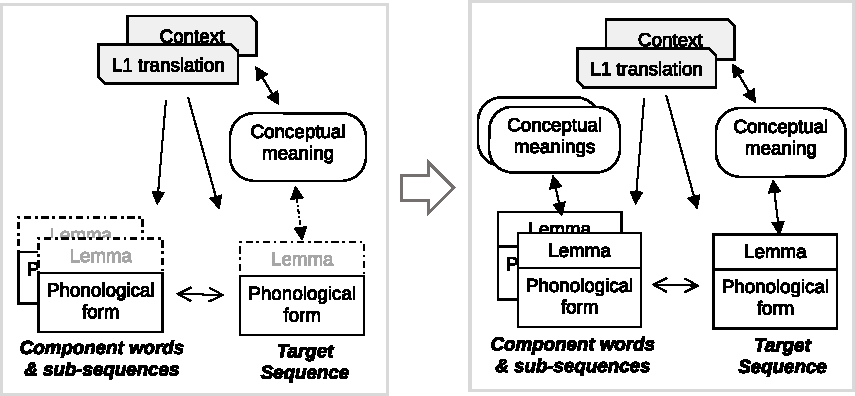
\includegraphics[width=\textwidth]{figures/cutlerFig4.pdf}
\end{figure}

\figref{fig:cutler:4} presents a highly simplified model of this process, showing possible initial and final stages in the holistic acquisition of a formulaic expression. Initially, hearing the expression in context and seeing the L1 translation help set up the conceptual meaning. The holistic phonological form is established through the DR process and linked to the concept (and the strength of this may vary, as shown by the dotted arrow). The phonological form may also be linked associatively with phonological forms of words and sub-sequences, but direct links to their meanings are discouraged. As the target is retrieved and repeated over time, the link between the concept and the lemma are strengthened along with associative links to the lemmas of the component words and sub-sequences. This consolidates the holistic sequence lemma in memory and helps make it easier to recall

\subsubsection{Modelling fusion}


There were also cases of apparent ``fusion'', where a sequence was initially reconstructed to some extent before later becoming formulaic. In many of these cases, components and sub-sequences (e.g. \textit{breathed} and \textit{sigh of relief}); \textit{turned} and \textit{blind eye}) appear to be combined on-line, with dysfluencies marking their joins. In some cases, errors occur at the joins (\textit{breathed his sigh of relief}; \textit{turned blind eye}) usually involving less salient function words (e.g. \textit{a}, \textit{to}), or occasionally with the wrong choice of lexical word (e.g. \textit{set his mind on}). There were also examples of morphological changes to the key lexical words (\textit{breathe}; \textit{turn}) compared to the given target. The morphological and lexical changes suggest that the meanings of the component words were being accessed during the reconstruction. Fusion therefore seems to involve a combination of the chunking together of known components and the correcting of erroneous or missing words. To some extent this process mirrors the latter stages of a sequence postulated by Bardovi-Harlig (2019, p.110) for the pragmatic L2 acquisition of ``conventional expressions'': 

\begin{quote}
nontargetlike response → target-like response but non-target-like lexical resources → target-like lexical core → full conventional expression
\end{quote}

In the fusion cases of the current study, the targeted learning of given expressions appears to move learners quickly to the ``target-like lexical core'' stage, but further development is required to become fully formulaic. A possible model for this fusion process is given in \figref{fig:cutler:5}.


\begin{figure}
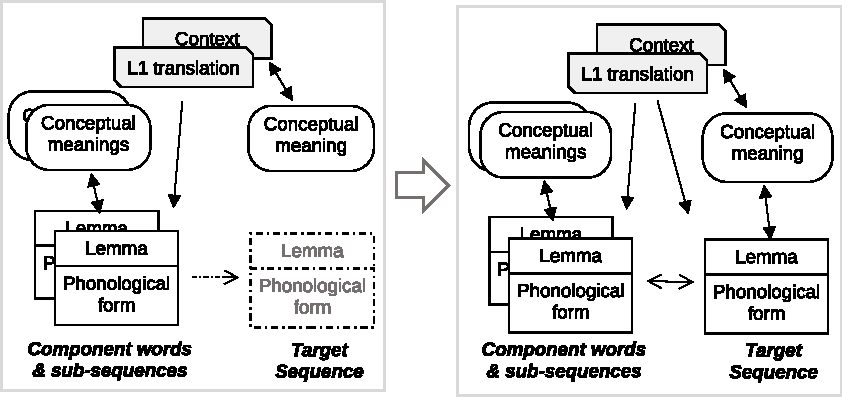
\includegraphics[width=\textwidth]{figures/cutlerFig5.pdf}
\caption{Simple model of fusion for L2 speakers. Arrows with filled heads show meaning relationship, those with non-filled show associative links\slash co-activation. Dotted arrows indicate weaker links\slash dotted boxes indicate empty elements.\label{fig:cutler:5}}
\end{figure}


In the initial learning stage, while a conceptual meaning for the target expression may be established, it is not linked to a holistic lemma or single phonological form. To recreate the expression therefore, it is necessary to access the lemmas of the component words and sub-sequences which have been linked to the context and L1 translation (possibly via their conceptual meanings).  So, while an ``empty'' expression lemma may be created, it takes further retrieval and repetition to facilitate the chunking up and correcting required to develop a fused phonological form. 

\subsection{Conclusion}

The two studies showed clear differences in the effect of the different learning approaches on internal formulaicity, along with useful insights into the acquisition process. However, it should be acknowledged that the number of participants and target sequences tested is relatively small and representative of a specific type of learner and formulaic expression. For this reason, the research presented should be seen as exploratory and the results and conclusions would ideally be verified through larger scale studies and different types of learner. It is also important to emphasise that the approach and discussion focus on a particular definition of internal formulaicity and specific means of identifying it.

With those caveats in mind, the studies do nevertheless demonstrate that both holistic acquisition and fusion (as described here) are two possible routes for a target expression to become internally formulaic for a speaker. They further suggest that the method by which targets are memorised influences which of these routes is taken. Figures~\ref{fig:cutler:5} and~\ref{fig:cutler:6} show a possible way of modelling these route which are consistent with some existing models of lexical acquisition. They also show how apparently ``partial'' formulaicity may be compatible with a model based on the idea of holistic storage. A particular implication is that, in the case of fusion, the meanings of component words and sequences are accessed in order to construct the expression, while this is not necessary for holistic acquisition. Fusion is therefore likely to be more susceptible to interference based on the speaker’s existing knowledge of the component words or sub-sequences. Examples of this from the studies include cases where words may be strongly linked to other similar expressions (e.g. \textit{like the idea of} for \textit{like the sound of}) or when synonyms replace component words (e.g. \textit{set his target on}). It also suggests that part of the benefits (for formulaic acquisition) of an approach such as Dynamic Repetition (DR) is that it de-emphasises the meanings of the component words. This is certainly beneficial in expressions where, like the targets in the studies, the whole is not (semantically) the sum of the parts. 

With DR, the focus on repetition of the whole (delivered with sufficient intonation and feeling) may help to establish holistic storage of sequences early on, and maintain fluency and formulaicity of output over time. Further, because the whole is sufficiently linked to a particular example context and meaning, the simple repetition does not appear to impact negatively on recall or accuracy compared to the semantic-formal elaboration (SFE). While it was not designed as a pedagogic tool, DR in combination with certain elaborative approaches such as drawing attention to prosodic features of target sequences \citep{BoersEtAl2012} may be a useful way of promoting formulaic acquisition. The studies also support the idea of regular (spaced) retrieval and simple corrective feedback as a way of consolidating recall and formulaicity of the learnt sequences.

Along with the way expressions are memorised, there are likely to be many other factors which could influence the extent to which target expressions will become formulaic for a speaker and the route taken to do so. Indeed, despite the controlled choice of participants and sequences in the studies, there was still considerable variation in performance across participants and sequences. However, rather than any systematic trends for particular features of sequences (e.g. length) or participant (e.g. proficiency level), any variation appears more likely to be a complex interaction between these, related in part to the speaker’s particular experience with the words and sub-sequences of each sequence. Further research which manipulates known or unknown component words and sub-sequences within target sequences when being learnt by L2 speakers may be useful to explore the routes to formulaicity further. It would also be interesting to investigate how other variables (such as length, prosodic features, imageability and L1 congruence) may affect these routes.


{\sloppy\printbibliography[heading=subbibliography,notkeyword=this]}
\end{document}
